\documentclass[tikz,border=8pt]{standalone}
\usepackage{amsmath,amssymb}
\usetikzlibrary{arrows.meta,calc,decorations.pathreplacing,decorations.markings,decorations.pathmorphing,patterns,shapes.geometric,positioning,shadings,plotmarks}

\begin{document}
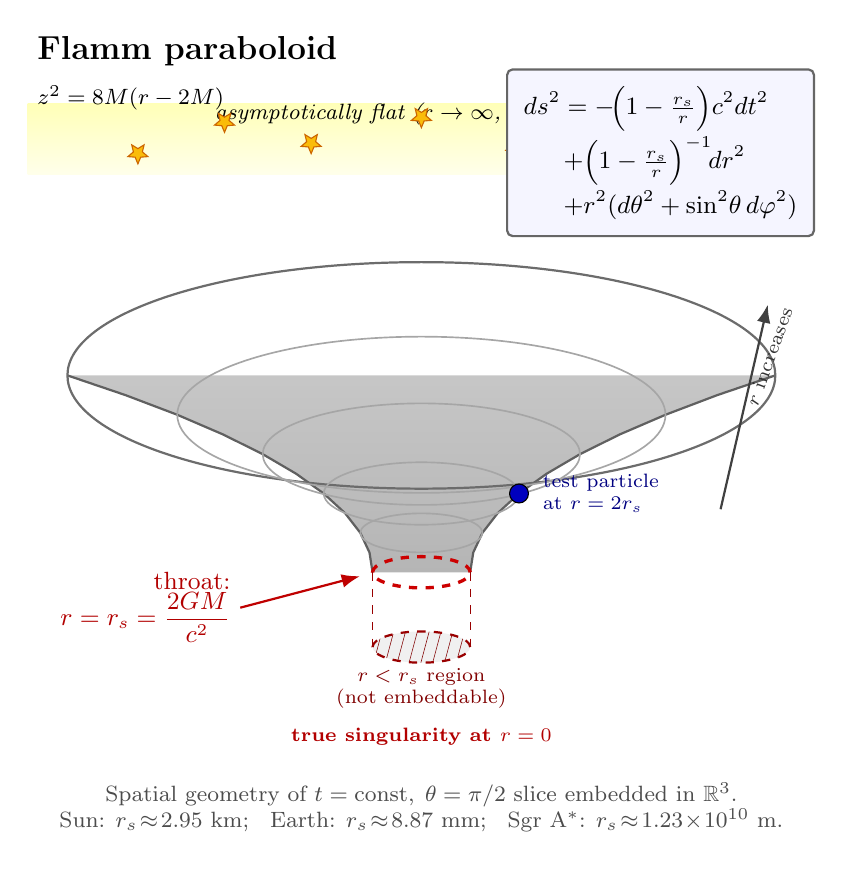
\begin{tikzpicture}[>=Latex,font=\sffamily]

  % =========================================================================
  % Flamm paraboloid embedding of the Schwarzschild t=const, theta=pi/2 slice
  % Profile: z(r) = 2 sqrt(r_s (r - r_s)).  r_s = 1 in figure units.
  % We render with a side-view: x_canvas = 0.62 * (+/- r), y_canvas = 0.50 * z.
  % =========================================================================

  % --- Foreshortening factor for ring ellipses
  \pgfmathsetmacro{\fore}{0.32}

  % --- Top: asymptotic flat halo (pale yellow band) ------------------------
  \shade[top color=yellow!28, bottom color=yellow!8]
    (-5.0, 5.05) rectangle (5.0, 5.95);
  \node[font=\footnotesize\itshape, anchor=south] at (0, 5.55)
    {asymptotically flat ($r\to\infty$, Minkowski)};
  \foreach \x/\y in {-3.6/5.32, -2.5/5.72, -1.4/5.45, 0.0/5.78, 1.2/5.40,
                     2.4/5.70, 3.5/5.30} {
    \node[star, star points=5, star point ratio=0.45,
          fill=yellow!50!orange, draw=orange!80!black,
          inner sep=0pt, minimum size=0.12cm] at (\x, \y) {};
  }

  % --- Build coordinate path nodes for the paraboloid silhouette -----------
  % At z values 0,0.5,1.0,...,5.0 we have x = 0.62 * (1 + z^2/4).
  % We define them as named coordinates.
  \foreach \i/\z in {0/0.0, 1/0.5, 2/1.0, 3/1.5, 4/2.0, 5/2.5,
                     6/3.0, 7/3.5, 8/4.0, 9/4.5, 10/5.0}{
    \pgfmathsetmacro{\rzz}{1.0 + (\z * \z) / 4.0}
    \pgfmathsetmacro{\xv}{0.62 * \rzz}
    \pgfmathsetmacro{\yv}{0.50 * \z}
    \coordinate (R\i) at (\xv, \yv);
    \coordinate (L\i) at (-\xv, \yv);
  }

  % --- Filled silhouette (gray gradient) -----------------------------------
  \begin{scope}
    \clip (L10) -- (L9) -- (L8) -- (L7) -- (L6) -- (L5) -- (L4) -- (L3)
       -- (L2) -- (L1) -- (L0) -- (R0) -- (R1) -- (R2) -- (R3) -- (R4)
       -- (R5) -- (R6) -- (R7) -- (R8) -- (R9) -- (R10) -- cycle;
    \shade[top color=gray!28, bottom color=gray!58]
      (-4.5, 0) rectangle (4.5, 5.5);
  \end{scope}

  % --- Outline (left + right curves) ---------------------------------------
  \draw[gray!75!black, thick]
    (L10) -- (L9) -- (L8) -- (L7) -- (L6) -- (L5) -- (L4) -- (L3)
       -- (L2) -- (L1) -- (L0);
  \draw[gray!75!black, thick]
    (R10) -- (R9) -- (R8) -- (R7) -- (R6) -- (R5) -- (R4) -- (R3)
       -- (R2) -- (R1) -- (R0);

  % --- Top mouth ellipse (mouth of the funnel, r large) --------------------
  \pgfmathsetmacro{\rztop}{1.0 + (5.0 * 5.0) / 4.0}        % 7.25
  \pgfmathsetmacro{\xtop}{0.62 * \rztop}                    % 4.495
  \pgfmathsetmacro{\ytop}{\fore * \xtop}                    % ~1.438
  \draw[gray!85!black, thick] (0, 2.5) ellipse [x radius=\xtop, y radius=\ytop];

  % --- Intermediate latitude rings -----------------------------------------
  \foreach \z in {4.0, 3.0, 2.0, 1.0}{
    \pgfmathsetmacro{\rzz}{1.0 + (\z * \z) / 4.0}
    \pgfmathsetmacro{\xrad}{0.62 * \rzz}
    \pgfmathsetmacro{\yrad}{\fore * \xrad}
    \pgfmathsetmacro{\ycen}{0.50 * \z}
    \draw[gray!70, semithick] (0, \ycen) ellipse [x radius=\xrad, y radius=\yrad];
  }

  % --- Throat ring (r = r_s): RED DASHED -----------------------------------
  \pgfmathsetmacro{\xbot}{0.62}
  \pgfmathsetmacro{\ybot}{\fore * \xbot}
  \draw[red!80!black, very thick, dashed] (0, 0) ellipse [x radius=\xbot, y radius=\ybot];

  % --- Below throat: shaded "interior" region (not embeddable) ------------
  \begin{scope}
    \clip (0, -0.95) ellipse [x radius=\xbot, y radius=\ybot];
    \fill[gray!12] (-1.5, -1.6) rectangle (1.5, 0);
    \foreach \xx in {-0.7, -0.55, -0.4, -0.25, -0.1, 0.05, 0.2, 0.35, 0.5}{
      \draw[red!50!black, very thin] (\xx, -1.5) -- (\xx + 0.4, 0);
    }
  \end{scope}
  \draw[red!60!black, dashed, thick] (0, -0.95) ellipse [x radius=\xbot, y radius=\ybot];
  \draw[red!60!black, thin, dashed] (-\xbot, 0) -- (-\xbot, -0.95);
  \draw[red!60!black, thin, dashed] (\xbot, 0)  -- (\xbot, -0.95);
  \node[font=\scriptsize, anchor=north, text=red!50!black, align=center]
    at (0, -1.10) {$r<r_s$ region\\(not embeddable)};
  \node[font=\scriptsize\bfseries, anchor=north, text=red!70!black, align=center]
    at (0, -1.85) {true singularity at $r=0$};

  % --- Test particle on the paraboloid at z=2 (r = 2 r_s) -----------------
  \pgfmathsetmacro{\zP}{2.0}
  \pgfmathsetmacro{\rP}{1.0 + (\zP * \zP) / 4.0}     % 2.0
  \pgfmathsetmacro{\xP}{0.62 * \rP}                   % 1.24
  \pgfmathsetmacro{\yP}{0.50 * \zP}                   % 1.0
  \fill[blue!75!black] (\xP, \yP) circle (0.12);
  \draw[black] (\xP, \yP) circle (0.12);
  \node[font=\scriptsize, anchor=west, text=blue!50!black, align=left]
    at (\xP+0.18, \yP) {test particle\\at $r=2 r_s$};

  % --- Throat label --------------------------------------------------------
  \draw[->, thick, red!75!black] (-2.30, -0.45) -- (-0.78, -0.05);
  \node[font=\small, anchor=east, text=red!70!black, align=right]
    at (-2.30, -0.45) {throat:\\$r = r_s = \dfrac{2GM}{c^{2}}$};

  % --- "Flamm paraboloid" title label --------------------------------------
  \node[font=\large\bfseries, anchor=south west] at (-5.0, 6.30)
    {Flamm paraboloid};
  \node[font=\footnotesize\itshape, anchor=north west] at (-5.0, 6.30)
    {$z^{2}=8M(r-2M)$};

  % --- Metric formula box (top-right) --------------------------------------
  \node[draw=black!60, thick, rounded corners=2pt, fill=blue!4,
        inner sep=6pt, anchor=north east, align=left, font=\small]
    at (5.0, 6.40)
    {$\displaystyle ds^{2}=-\!\Bigl(1-\tfrac{r_s}{r}\Bigr)c^{2}dt^{2}$\\[1pt]
     $\displaystyle \quad\;\;+\Bigl(1-\tfrac{r_s}{r}\Bigr)^{-1}\!dr^{2}$\\[1pt]
     $\displaystyle \quad\;\;+r^{2}(d\theta^{2}+\sin^{2}\!\theta\,d\varphi^{2})$};

  % --- Arrow indicating "r increases outward along the surface" -----------
  \draw[->, thick, gray!50!black] (3.8, 0.8) -- (4.4, 3.4);
  \node[font=\scriptsize, anchor=west, text=gray!40!black, rotate=70]
    at (4.15, 2.0) {$r$ increases};

  % --- Bottom note: numerical r_s for Sun, Earth, Sgr A* -------------------
  \node[font=\footnotesize, anchor=north, align=center, text=black!70]
    at (0, -2.55)
    {Spatial geometry of $t=\text{const},\;\theta=\pi/2$ slice
     embedded in $\mathbb{R}^{3}$.\\
     Sun: $r_{s}\!\approx\!2.95$ km;\;\;
     Earth: $r_{s}\!\approx\!8.87$ mm;\;\;
     Sgr A$^{*}$: $r_{s}\!\approx\!1.23\!\times\!10^{10}$ m.};

\end{tikzpicture}
\end{document}
